\chapter{ Констукторский раздел}
\label{cha:design}

В данном разделе мы рассмотрим схемы вышеизложенных алгоритмов.

\section{Разработка алгоритмов}

\begin{figure}[ht!]
	\centering{
		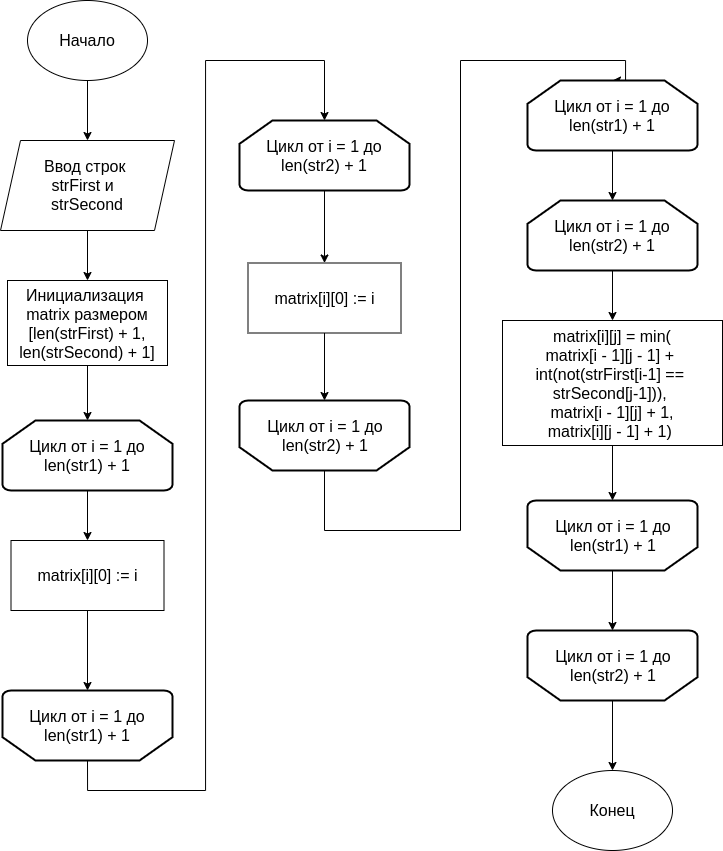
\includegraphics[width=0.6\textwidth]{img/diagramLev.png}
		\caption{Схема алгоритма Левенштейна}
		\label{fg:ref1}}
\end{figure}


\begin{figure}[ht!]
	\centering{
		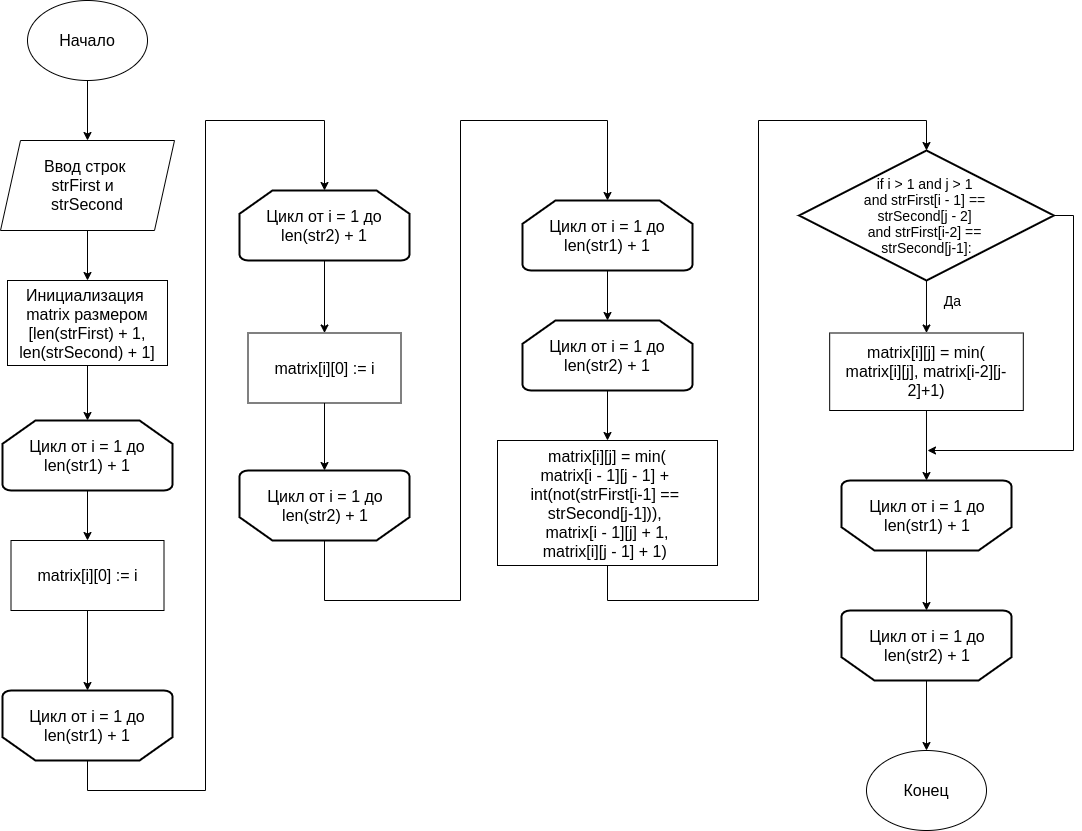
\includegraphics[width=1\textwidth]{img/diagramDamLev.png}
		\caption{Схема алгоритма Дамерау-Левенштейна}
		\label{fg:ref2}}
\end{figure}

\begin{figure}[ht!]
	\centering{
		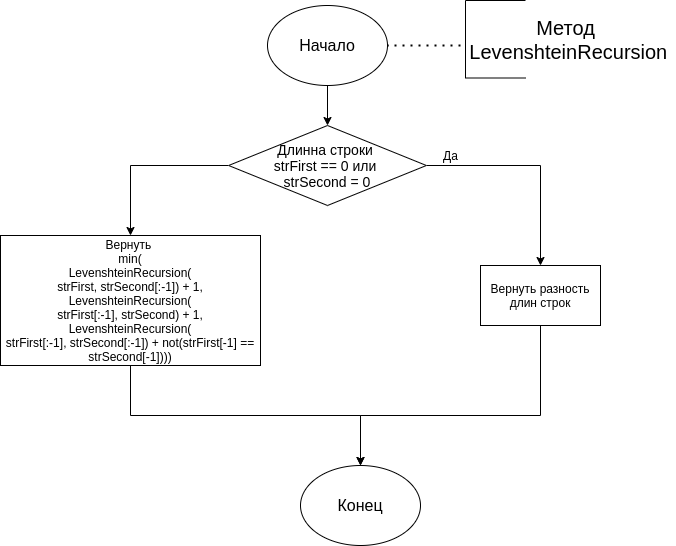
\includegraphics[width=0.8\textwidth]{img/diagramLevRec.png}
		\caption{Схема рекурсивного алгоритма Левенштейна}
		\label{fg:ref3}}
\end{figure}

\section{Вывод}

В данном разделе мы рассмотрели схемы алгоритмов Левенштейна (\ref{fg:ref1}). и Дамерау-Левенштейна (\ref{fg:ref2}).






